\documentclass[hyperref={breaklinks,colorlinks}]{beamer}
% \usepackage[UTF8,noindent]{ctex}
\usepackage{amsmath,amsxtra} \usepackage{color}
\usefonttheme[onlymath]{serif}
% \usepackage{fontspec}
\usepackage[version=3]{mhchem} \usepackage{fixltx2e}
\usepackage[customcolors]{hf-tikz} \usepackage{xcolor}
\usepackage{lmodern} \usepackage{listings}

\lstset{ numbersep=-10pt, basicstyle=\ttfamily,
  keywordstyle=\color{red}, commentstyle=\color{gray},
  morecomment=[l]{!\ },% Comment only with space after !
  frame=shadowbox, basicstyle=\tiny,
  rulesepcolor=\color{red!20!green!20!blue!20}, }

\usepackage{attachfile}

\usetheme{CambridgeUS} \usecolortheme{orchid}

% \usepackage{capt-of} CTeX fontset `fandol' is unavailable in current
% mod
\usepackage{lmodern} % remove the warning for use of the \textit
\makeatletter \renewcommand\normalsize{%
  \@setfontsize\normalsize\@xpt\@xiipt \abovedisplayskip 1\p@
  \@plus2\p@ \@minus5\p@ \abovedisplayshortskip \z@ \@plus3\p@
  \belowdisplayshortskip 6\p@ \@plus3\p@ \@minus3\p@ \belowdisplayskip
  \abovedisplayskip \let\@listi\@listI} \makeatother
\setbeamerfont{caption}{size=\tiny} \title{Build the topology of ion }
\author{Zhang Haomiao } \institute{HUST} \date{\today}
\setlength\abovecaptionskip{0pt}
\begin{document}
\frame{\maketitle} \frame{\tableofcontents{}}
\section{PREPARE PDB}
\begin{frame}  
  \frametitle{PDB and mol2 file}
  AMBER NAMING scheme for residues \textcolor{red}{HID HIE HIP
    $\rightarrow$ HIS}

  Prepare \textbf{mol2} file for non--standard residues
  \begin{block}{PDB ID: 1OKL}
    3 His residues and 1
    MNS((5-(DimethyLamino)-1-Naphthalenesulfonamide)) ligand in its
    metal site
  \end{block}
  \begin{itemize}
  \item Make sure no atoms use the same atom name in a certain
    residue, manually correct it before processing
  \item Make sure the residue name and atom name of the metal ion are
    all capitalized
  \item Make sure each metal ion or halide ion is treated separately
    as independent residue
  \end{itemize}
\end{frame}


\begin{frame}[t,fragile]
  \frametitle{Ligand file}
  \begin{enumerate}
  \item Use \textit{\textbf{reduce}} in AmberTools to add hydrogens to
    ligands. (GaussainView for manually).
\begin{lstlisting}
reduce MNS.pdb > MNS_H.pdb
\end{lstlisting}
  \item Delete the hydrogens which connect to the ligating nitrogen
    atom of zinc ion.  >> \underline{\texttt{MNS\_fixed\_H.pdb}} %% remove HN32
  \item Use \textit{\textbf{antechamber}} to generate mol2 file for
    non\_standard residues.

    (\texttt{AM1-BCC} to generate the charges, ligand has a charge -1
    , \texttt{GAFF} atom types)
\begin{lstlisting}
antechamber -fi pdb -fo mol2 -i MNS_fixed_H.pdb -o MNS_pre.mol2 -c bcc -pf y -nc -1 
\end{lstlisting}
    Note there is no "du" atom type in MNS\_pre.mol2 file , rename it
    to \underline{\texttt{MNS.mol2}}
  \item Perform the following command to obtain frcmod file for ligand
\begin{lstlisting}
parmchk2 -i MNS.mol2 -o MNS.frcmod -f mol2 
\end{lstlisting}
    Please make sure there is one and only one blank line after each
    parameter section >> \underline{\texttt{MNS.frcmod}}
  \end{enumerate}
\end{frame}

\begin{frame}[fragile]
  \frametitle{Metal ion and water}

  \begin{enumerate}
  \item Copy Zn ion into one single PDB file
    (\underline{\texttt{ZN.pdb}})
  \item Use \textbf{\textit{antechamber}} to generate mol2 file
\begin{lstlisting}
antechamber -fi pdb -fo mol2 -i ZN.pdb -o ZN_pre.mol2 -at amber -pf y 
\end{lstlisting}
  \item Change the atom type and charge in the \texttt{ZN\_pre.mol2}
    file, treat Zinc ion with atom "ZN" and charge 2.0 >>
    \texttt{\underline{ZN.mol2}}
  \item Keep crystal water during modeling, copy it into
    \texttt{WAT.pdb}
  \item Use \textit{\textbf{tleap} }to add hydrogen atoms to water
\begin{lstlisting}
tleap -s -f wat_tleap.in > wat_tleap.out 
\end{lstlisting}
  \item use \textit{\textbf{antechamber}} to generate mol2 files for
    water molecules.Using AMBER atom types
\begin{lstlisting}
antechamber -fi pdb -fo mol2 -i WAT_H.pdb -o WAT.mol2 -at amber -c bcc -pf y 
\end{lstlisting}
    >> \underline{\texttt{WAT\_H.pdb WAT.mol2}}
  \end{enumerate}
\end{frame}
\begin{frame}[fragile]
  \frametitle{Combine PDB files into PDB file}
  \begin{enumerate}
    \item use the webserver H++ to add hydrogen atoms to the PDB file,
      H++ will delete the non-standard residues during the modeling
      process, this PDB file will use an AMBER naming scheme for the
      residues.
\begin{lstlisting}
ambpdb -p 0.15_80_10_pH6.5_1OKL.top -c 0.15_80_10_pH6.5_1OKL.crd > 1OKL_Hpp.pdb
\end{lstlisting}
  \item Palce the standard residues, metal ion , ligand and water
  \item use cat to combine the pdb file
\begin{lstlisting}
cat 1OKL_Hpp_fixed.pdb ZN.pdb MNS_H_fixed.pdb > 1OKL_H.pdb
\end{lstlisting}
  \item using \texttt{\textbf{pdb4amber}} to renumber PDB file
\begin{lstlisting}
 pdb4amber -i 1OKL_H.pdb -o 1OKL_fixed_H.pdb
\end{lstlisting}
  \end{enumerate}
  >> PDB file : \texttt{\underline{1OKL\_fixed\_H.pdb}}\newline >>
  mol2 file \texttt{\underline{MNS.mol2 ZN.mol2}}
\end{frame}
\section{Generate PDB,Gaussian,GAMESS\_US and fingerprint modeling}
\begin{frame}
  \frametitle{Workflow of MCPB.py}
  {\centering
  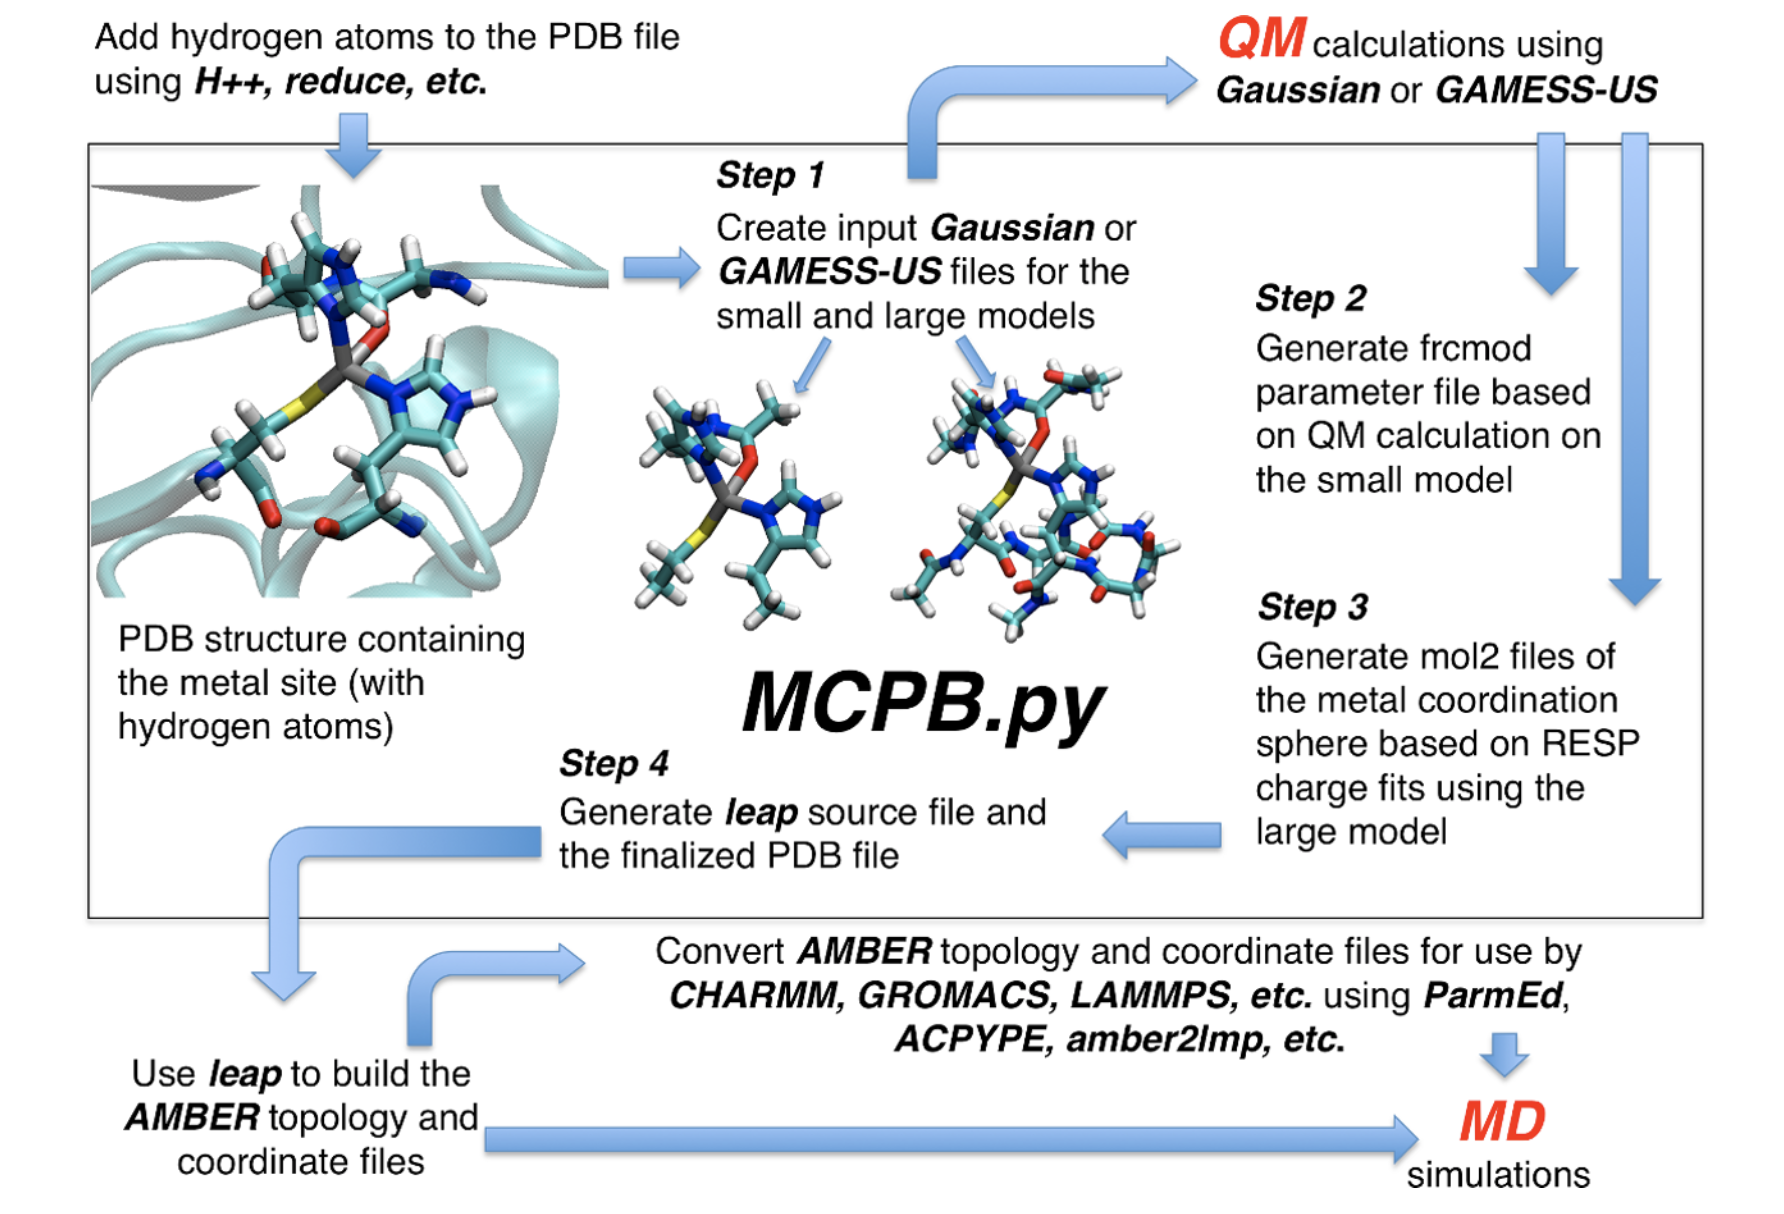
\includegraphics[scale=.35]{step.png}\par}
\end{frame}

\begin{frame}[fragile]

  \begin{enumerate}
    \frametitle{Generate file}
  \item INPUT FILE : 1OKL.in , using Gaussian09 , add
    "software\_version g09" as a line into the input file
    \begin{itemize}
    \item large\_opt equal 1 to optimize the hydrogen postions of the
      large model
    \item
\begin{lstlisting}
MCPB.py -i 1OKL.in -s 1
\end{lstlisting}
    \item OUTPUT PDB,fingerprint files of small, standard and large
      models
    \item OUTPUT Gaussian input file of small and large models
    \end{itemize}
  \item Run Gaussian09, perform geometry optimization, force constant
    calculation
\begin{lstlisting}
g09 < 1OKL_small_opt.com > 1OKL_small_opt.log
g09 < 1OKL_small_fc.com > 1OKL_small_fc.log 
\end{lstlisting}
  \item generate fchk file for small model
\begin{lstlisting}
formchk 1OKL_small_opt.chk > 1OKL_small_opt.fchk 
\end{lstlisting}
  \item Perform the Merz-Kollman RESP charge calculation for the large
    model
\begin{lstlisting}
g09 < 1OKL_large_mk.com > 1OKL_large_mk.log 
\end{lstlisting}
  \end{enumerate}
\end{frame}
\section{Perform the final modeling}
\begin{frame}[fragile]
  \begin{itemize}
  \item \textbf{Seminario method} to generate force field parameters
\begin{lstlisting}
MCPB.py -i 1OKL.in -s 2
\end{lstlisting}
    >>\underline{\texttt{1OKL\_mcpbpy.frcmod}}
  \item use the ChgModB to perform the RESP charge fitting and
    generate the mol2 files for the metal site residues
\begin{lstlisting}
MCPB.py -i 1OKL.in -s 3
\end{lstlisting}
    >>\underline{\texttt{ HD1.mol2, HD2.mol2, HE1.mol2, ZN1.mol2
        MS1.mol2}}
  \item Using mol2 file in leap modeling,generate tleap input file
\begin{lstlisting}
MCPB.py -i 1OKL.in -s 4
\end{lstlisting}
    >>\underline{\texttt{1OKL\_mcpbpy.pdb, 1OKL\_tleap.in}}
  \item use tleap to generate the topology and coordinate files
\begin{lstlisting}
tleap -s -f 1OKL_tleap.in > 1OKL_tleap.out
\end{lstlisting}
    >> \underline{\texttt{1OKL\_solv.prmtop, 1OKL\_solv.inpcrd}}
  \end{itemize}
\end{frame}
\begin{frame}[fragile]
  \frametitle{Check the modeling}
  \begin{itemize}
  \item use VMD to do a check about whether the coordiante bonds to
    metal ion exist in the topology file select
    \textbf{Graphics$\rightarrow$Representations},type same
    \textbf{residue as within 3 of resname ZN1},if all the four
    coordination bonds to zinc ion, then the outcome is correct.
  \item use cpptraj to do a check about the atom numbering issue
\begin{lstlisting}
cpptraj -p 1OKL_solv.prmtop
\end{lstlisting}
  \item Finally,use ParmEd to check the metal site parameters
\begin{lstlisting}
parmed -i mcpbpy_parmed.in -p 1OKL_solv.prmtop
\end{lstlisting}

    \begin{itemize}
     \only<1>{ \item[A)] The bond force constants between an metal ion and its
        ligating atoms are less than 200 kcal/(mol*Angstrom\^2), and the
        eqlibirum bond distances are less than 2.8 Angstrom;}
     \only<1>{ \item[B)] The angle force constants related to the metal ion are
        usually less than 100 kcal/(mol*Rad\^2) while the equlibirum angle
        values are bigger than 100 Degree;}
      \only<1>{\item[C)] All or most of the dihedral potential barriers are zero
        for metal involved dihedrals;}
      \only<2>{\item[D)] The RESP charge of the metal ion are less than its
        oxidation state, usually even less than +1;}
     \only<2>{ \item[E)] The LJ Radius of one metal ion is usually bigger than
        1.0 Angstrom.}
      \end{itemize}
  \end{itemize}
\end{frame}

\end{document}

%%% Local Variables:
%%% mode: latex
%%% TeX-master: t
%%% TeX-engine: luatex
%%% End:
